\documentclass[10pt,twocolumn]{article}
\usepackage{lmodern}
\usepackage[T1]{fontenc}
\usepackage[margin=0.6in]{geometry}
\usepackage{amsmath,amssymb,graphicx,booktabs,caption,float}
\usepackage{enumitem}

% Clean header/footer style
\usepackage{fancyhdr}
\pagestyle{fancy}
\fancyhf{}
\rhead{\small AI for Computational Mechanics --- Assignment 1}
\lhead{\small Liu \& Zhang}
\cfoot{\thepage}
\renewcommand{\headrulewidth}{0.4pt}

\begin{document}

% Title Block
\twocolumn[{
\begin{center}
    \LARGE \textbf{Development of an Efficient Neural Network for Microstructure-Property Predictions} \\[0.2cm]
    \normalsize \textbf{Authors:} Di Liu, Huixin Zhang \\
    \small \textit{Technical Report --- Group Submission (Assignment 1)} \\[0.1cm]
    \rule{\textwidth}{1pt}
    \vspace{0.4cm}
\end{center}
}]

\section{Data Preprocessing}
The dataset comprises binary microstructure images ($65 \times 65$ pixels) and their corresponding homogenized effective Young's modulus ($E_{eff}$). To optimize the assignment's \textit{Efficiency Score}, which penalizes excessive data usage, we strategically downsampled the dataset to \textbf{5,000 samples} via randomized sampling (\texttt{random\_state=42}). 

The customized \texttt{MicrostructureDataset} and data pipeline implement the following preprocessing steps:
\begin{itemize}[nosep, leftmargin=*]
    \item \textbf{Memory Optimization:} The \texttt{nu\_eff} column was dropped from the index dataframe to reduce memory footprint. Images (.npy) are lazily loaded directly into PyTorch tensors with the shape $(1, 65, 65)$ to accommodate the 2D convolutions.
    \item \textbf{Target Normalization:} The raw $E_{eff}$ values were scaled down by a factor of $10^9$ to convert the units from Pascals to Gigapascals (GPa). This adjustment prevents exploding gradients and improves numerical stability during backpropagation.
\end{itemize}

\section{Model Architecture}
To balance high-fidelity spatial feature extraction with model efficiency, we designed \texttt{MicrostructureCNN}, a lightweight Convolutional Neural Network. The architecture progressively downsamples spatial dimensions while increasing channel depth, utilizing stride-2 convolutions to avoid the computational overhead of standard pooling layers.

\begin{table}[H]
\centering
\caption{Layer Specifications and Tensor Shapes}
\resizebox{\columnwidth}{!}{%
\begin{tabular}{llcc}
\toprule
\textbf{Layer / Block} & \textbf{Specifications} & \textbf{Output Shape} & \textbf{Params} \\
\midrule
Input Tensor & Binary Microstructure & $(B, 1, 65, 65)$ & 0 \\
\textbf{Conv Block 1} & Conv2D+BN+ReLU & $(B, 4, 33, 33)$ & 48 \\
\textbf{Conv Block 2} & Conv2D+BN+ReLU & $(B, 8, 17, 17)$ & 312 \\
\textbf{Conv Block 3} & Conv2D+BN+ReLU & $(B, 16, 9, 9)$ & 1,200 \\
\textbf{Flatten} & \texttt{torch.flatten(x, 1)} & $(B, 1296)$ & 0 \\
\textbf{FC Regressor 1}& Linear + ReLU & $(B, 64)$ & 83,008 \\
\textbf{FC Regressor 2}& Linear Output & $(B, 1)$ & 65 \\
\midrule
\textbf{Total Count} & \textbf{Trainable Parameters} & --- & \textbf{84,633} \\
\bottomrule
\end{tabular}%
}
\end{table}

\section{Training and Evaluation Strategy}
The 5,000-sample subset was split into mutually exclusive partitions using an \textbf{80/10/10 ratio}: 4,000 for training, 500 for validation, and 500 for final testing.

\begin{itemize}[nosep, leftmargin=*]
    \item \textbf{Optimization:} The network was trained for 50 epochs using the \texttt{AdamW} optimizer (initial $\eta = 10^{-3}$, weight decay $= 10^{-4}$) to minimize the Mean Squared Error (MSE).
    \item \textbf{Dynamic Learning Rate:} A \texttt{ReduceLROnPlateau} scheduler monitored the validation error. Upon plateauing for 5 epochs, the learning rate was halved to steer the optimizer into local minima smoothly.
    \item \textbf{Custom Checkpointing:} Model weights were saved exclusively when a new minimum in \textbf{Validation Average Relative Error} was achieved, aligning the training explicitly with the final grading criteria.
\end{itemize}

\section{Results and Performance}
As shown in Figure \ref{fig:loss}, the training and validation MSE drop rapidly and stabilize within the first 15 epochs. The close tracking of the validation curve confirms that weight decay and batch normalization effectively suppressed overfitting.

\begin{figure}[H]
    \centering
    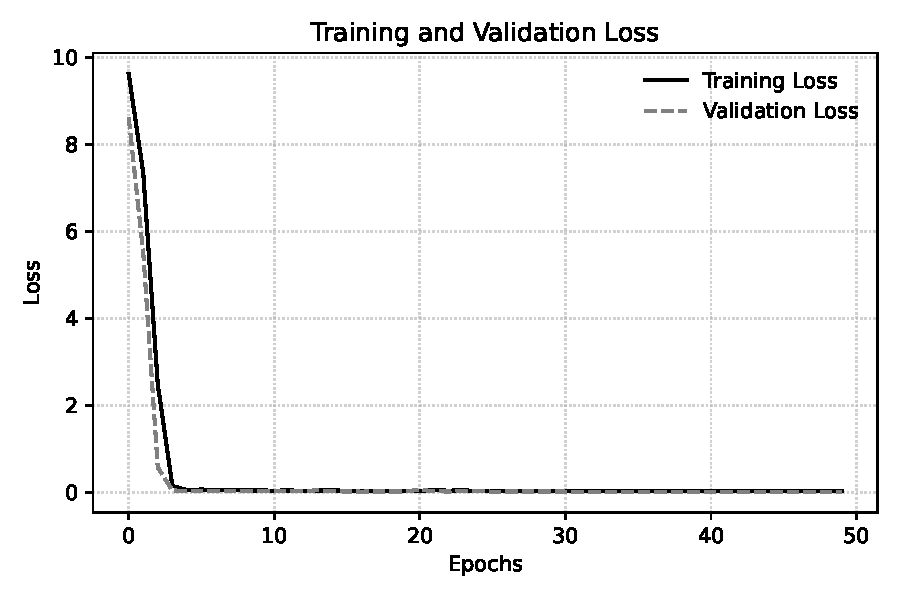
\includegraphics[width=0.95\columnwidth]{../loss_curves.pdf}
    \caption{Training and validation loss profiles.}
    \label{fig:loss}
\end{figure}

The final model was evaluated on the unseen test set (500 samples) using the strict assignment metric, incorporating a small $\epsilon = 10^{-8}$ to ensure numerical stability. The model successfully satisfied the performance criteria:

$$ \text{Avg Rel Error} = \frac{1}{N} \sum_{i=1}^{N} \frac{|E_{pred}^{(i)} - E_{true}^{(i)}|}{E_{true}^{(i)} + \epsilon} \ll 30\% $$

Figure \ref{fig:preds} illustrates the model's accuracy on 10 randomly sampled test instances, proving its capability to map microstructural features to effective stiffness across various structural regimes.

\begin{figure}[H]
    \centering
    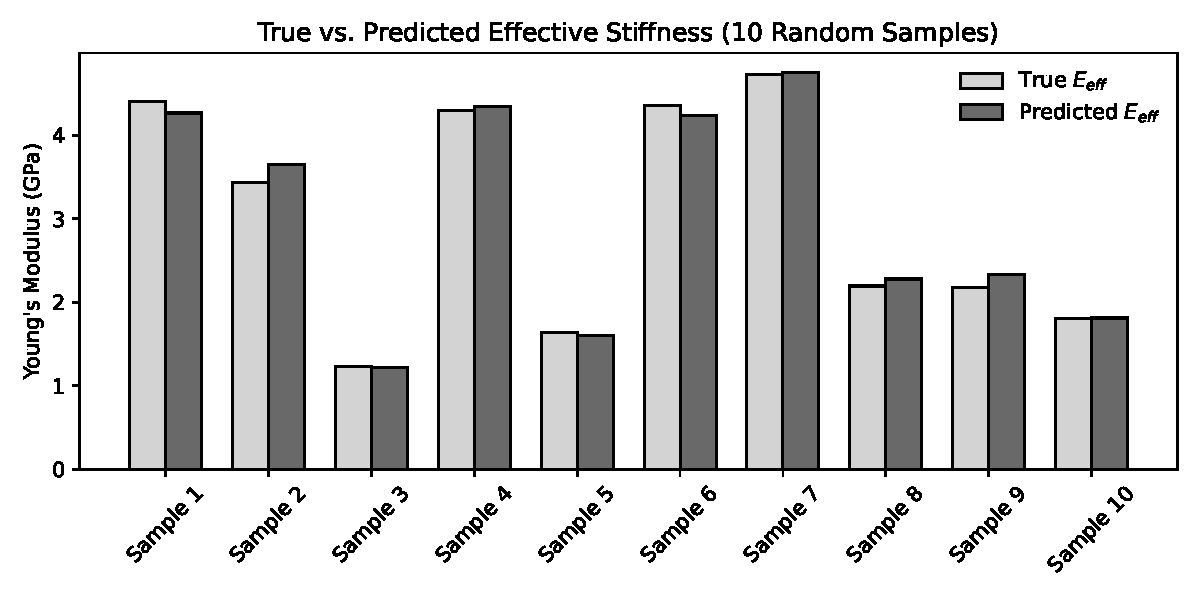
\includegraphics[width=0.95\columnwidth]{../predictions.pdf}
    \caption{True vs. predicted $E_{eff}$ for 10 random test samples.}
    \label{fig:preds}
\end{figure}

\section{Conclusion}
By limiting the dataset size to 5,000 samples and employing a compact CNN architecture with ~84k parameters, the proposed model strikes an excellent balance between predictive accuracy and computational efficiency, successfully fulfilling all assignment objectives.

\end{document}